\documentclass[]{../template/Report}
\settemplatedir{../template/} %设置模板文件夹路径
\exname{万用表的设计} %实验名称
\extable{}
\instructor{} %指导教师
\class{} %班级
\extable{}
\name{} %姓名
\stuid{} %学号

\nyear{2025} %年
\nmonth{9} %月
\nday{24} %日
\nweekday{三} %星期几
\daypart{上午} %上午/下午
\redate{} %如有实验补做,补做日期
\resitu{} %情况说明:

\begin{document}
\makecover

\section{预习报告}
\subsection{实验综述}
\subsubsection{测量电流计的内阻}
    利用替代法或中值法测量电流计内阻。这里使用替代法(\cref{tidaifa}),先将电流计与标准电流表同时串接在回路中。调节可变电阻使回路电流为合适大小$I_0$,再将电流计用电阻箱换下,调整电阻箱阻值,使回路电流仍为$I_0$,此时电阻箱的阻值即为电流计的内阻。
    \begin{figure}[htbp]
        \centering
        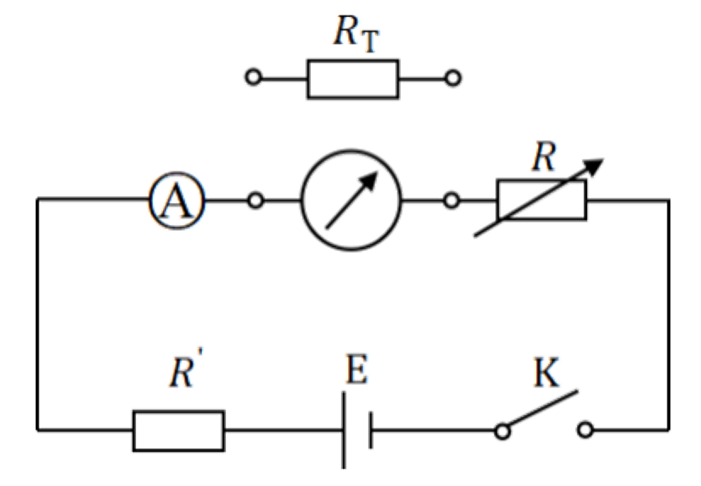
\includegraphics[width=0.4\textwidth]{tidaifa.png}
        \caption{替代法测量电流计内阻}
        \label{tidaifa}
    \end{figure}

\subsubsection{设计、改装并校准电流表}
    设计改装电流表电路如\cref{gaizhuangA}所示。由并联电压相等,根据改装后的量程$I_1 (\SI{5}{\milli A})$列出方程:
    \begin{equation}
        I_g R_g = (I_1 - I_g) R_1
    \end{equation}
    计算出$R_1 = \frac{I_g}{I_1-I_g} R_1$,将电阻箱调为对应阻值接入电路,得到改装电流表。

    然后,用\cref{jiaozhunA}所示电路校验并校准改装电流表,若测量值偏小,则增大电阻箱内阻,反之则减小电阻箱内阻,直至测量值与标准电流表读数相符。记录所得数据并分析误差。
    \begin{figure}[htbp]
        \centering
        \begin{subfigure}[b]{0.45\textwidth}
            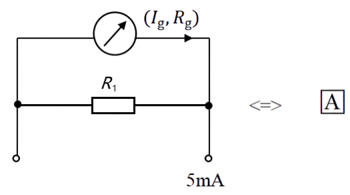
\includegraphics[width=\textwidth]{gaizhuangA.png}
            \caption{改装电流表设计电路}
            \label{gaizhuangA}
        \end{subfigure}
        \hfill
        \begin{subfigure}[b]{0.45\textwidth}
            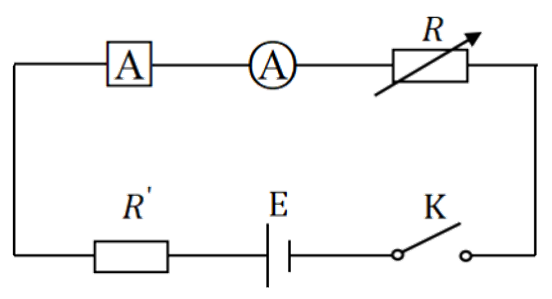
\includegraphics[width=\textwidth]{jiaozhunA.png}
            \caption{改装电流表校准电路}
            \label{jiaozhunA}
        \end{subfigure}
    \caption{改装电流表相关电路}
    \end{figure}

\subsubsection{设计、改装并校准电压表}
    设计改装电压表电路如\cref{gaizhuangV}所示。由串联电流相等,根据改装后的量程$U_1 (\SI{5}{V})$列出方程:
    \begin{equation}
        \begin{cases}
            (R_g'+R_3)I_g' = U_1\\
            R_g' = \frac{R_g R_1}{R_g + R_1} \\
            I_g' = I_1 
        \end{cases}
    \end{equation}
    计算出$R_3=\frac{U_1}{I_1} - \frac{R_g R_1}{R_g + R_1}$,将电阻箱调为对应阻值接入电路,得到改装电压表。

    然后,用\cref{jiaozhunV}所示电路校验并校准改装电压表,若测量值偏小,则减小电阻箱内阻,反之则增大电阻箱内阻,直至测量值与标准电压表读数相符。记录所得数据并分析误差。
    \begin{figure}[htbp]
        \centering
        \begin{subfigure}[b]{0.45\textwidth}
            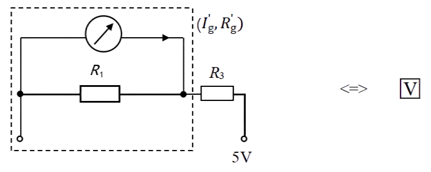
\includegraphics[width=\textwidth]{gaizhuangV.png}
            \caption{改装电压表设计电路}
            \label{gaizhuangV}
        \end{subfigure}
        \hfill
        \begin{subfigure}[b]{0.45\textwidth}
            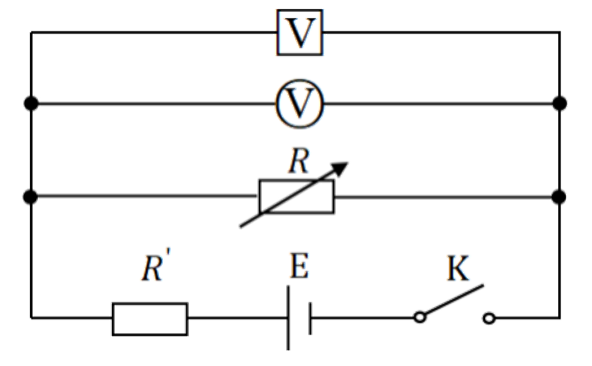
\includegraphics[width=\textwidth]{jiaozhunV.png}
            \caption{改装电压表校准电路}
            \label{jiaozhunV}
        \end{subfigure}
        \caption{改装电压表相关电路}
    \end{figure}

\subsubsection{改装欧姆表}
    设计欧姆表电路如\cref{gaizhuangOhm}所示。首先短接$a,b$,调节$R_6$使电流计满偏,此时有$I_o = I_g' = \frac{\varepsilon}{R_g'+R'}$,其中$R'$为回路中其他所有电阻之和。当不同$R_x$接入回路时,有$I_x = \frac{\varepsilon}{R_g'+R'+R_x}$,多次调节$R_x$记录$I_x$和$R_x$的值,并可在电流计面板上刻上刻度以显示不同阻值。特别地,当$I_x=\frac{I_o}{2}$时,有$R_x = R_g' + R'$称为欧姆表的中值电阻。
    \begin{figure}[htbp]
        \centering
        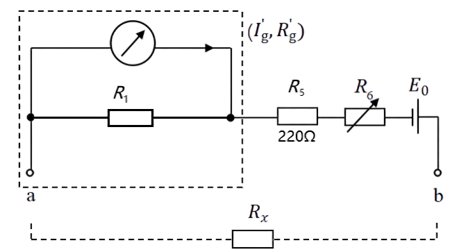
\includegraphics[width=0.4\textwidth]{gaizhuangOhm.png}
        \caption{欧姆表设计电路}
        \label{gaizhuangOhm}
    \end{figure}
\subsection{实验重点}
\begin{enumerate}
    \item 掌握电流计的工作原理及其内阻的测量方法;
    \item 学会电流表和电压表的设计、改装与校准方法;
    \item 理解欧姆表的工作原理及其改装方法。
\end{enumerate}
\subsection{实验难点}
\begin{enumerate}
    \item 设计改装电流表和电压表时,计算并调节电阻箱阻值以实现所需量程;
    \item 理解并应用误差分析方法,确保实验结果的准确性和可靠性;
    \item 正确应用电路连接和调试技巧,确保实验过程顺利进行;
    \item 正确进行实验设计和数据分析。
\end{enumerate}
\begin{fullreportonly}
% \section{原始数据}
%     \begin{figure}[H]
%         \centering
%         \includegraphics[width=0.9\textwidth]{rawdata_wanyongbiao.jpg}
%         \caption{原始数据}
%         \label{example_data}
%     \end{figure}

\section{结果与分析}
\subsection{数据处理与结果}
\subsubsection{测量电流计的内阻}
通过替代法,测得电流计内阻为$R_g = \SI{231}{\ohm}$。
\subsubsection{设计、改装并校准电流表}
经计算,$R_1 = \SI{57.7}{\ohm}$。由于改装后电流表分度值为$\frac{\SI{5}{\milli A}}{5 \times 10} = \SI{0.1}{\milli A}$,因此估读到$\SI{0.01}{\milli A}$。实验数据如\cref{tableA}所示,其中$\Delta I = I_{\text{标准}} - I_{\text{改装}}$。
\begin{table}[H]
  \centering
  \caption{改装$\SI{5}{\milli A}$电流表的实验数据}
  \begin{tabular}{C{.3\textwidth} *{5}{C{.11\textwidth}}}
    \toprule
    实验序号 & 1 & 2 & 3 & 4 & 5 \\
    \midrule
    $I_{\text{G}} / \si{mA}$ & 1.00 & 2.00 & 3.00 & 4.00 & 5.00 \\
    \midrule
    $I_{\text{B}} / \si{mA}$ & 1.02 & 1.96 & 2.98 & 4.01 & 4.99 \\
    \midrule
    $\Delta I / \si{mA}$        & 0.02 & -0.04 & -0.02 & 0.01 & -0.01 \\
    \midrule
    $\varepsilon_r$ & 2.00\% & 2.00\% & 0.67\% & 0.25\% & 0.20\% \\
    \midrule
    校准后的并联电阻$R_2 / \si{\ohm}$ &60.0 &60.0 &60.0 & 60.0 &60.0 \\
    \bottomrule
    \label{tableA}
  \end{tabular}
\end{table}
计算得$\Delta_{max} = \left| \frac{-0.04}{0.1}\right| = 0.4$,故改装电流表的等级为0.4。
改装后电流表的$I_G \sim I_B$曲线如\cref{releA}所示,$\Delta I \sim I_\text{校准}$曲线如\cref{deltaA}所示。
\begin{figure}[htbp]
    \centering
    \begin{subfigure}[b]{0.45\textwidth}
        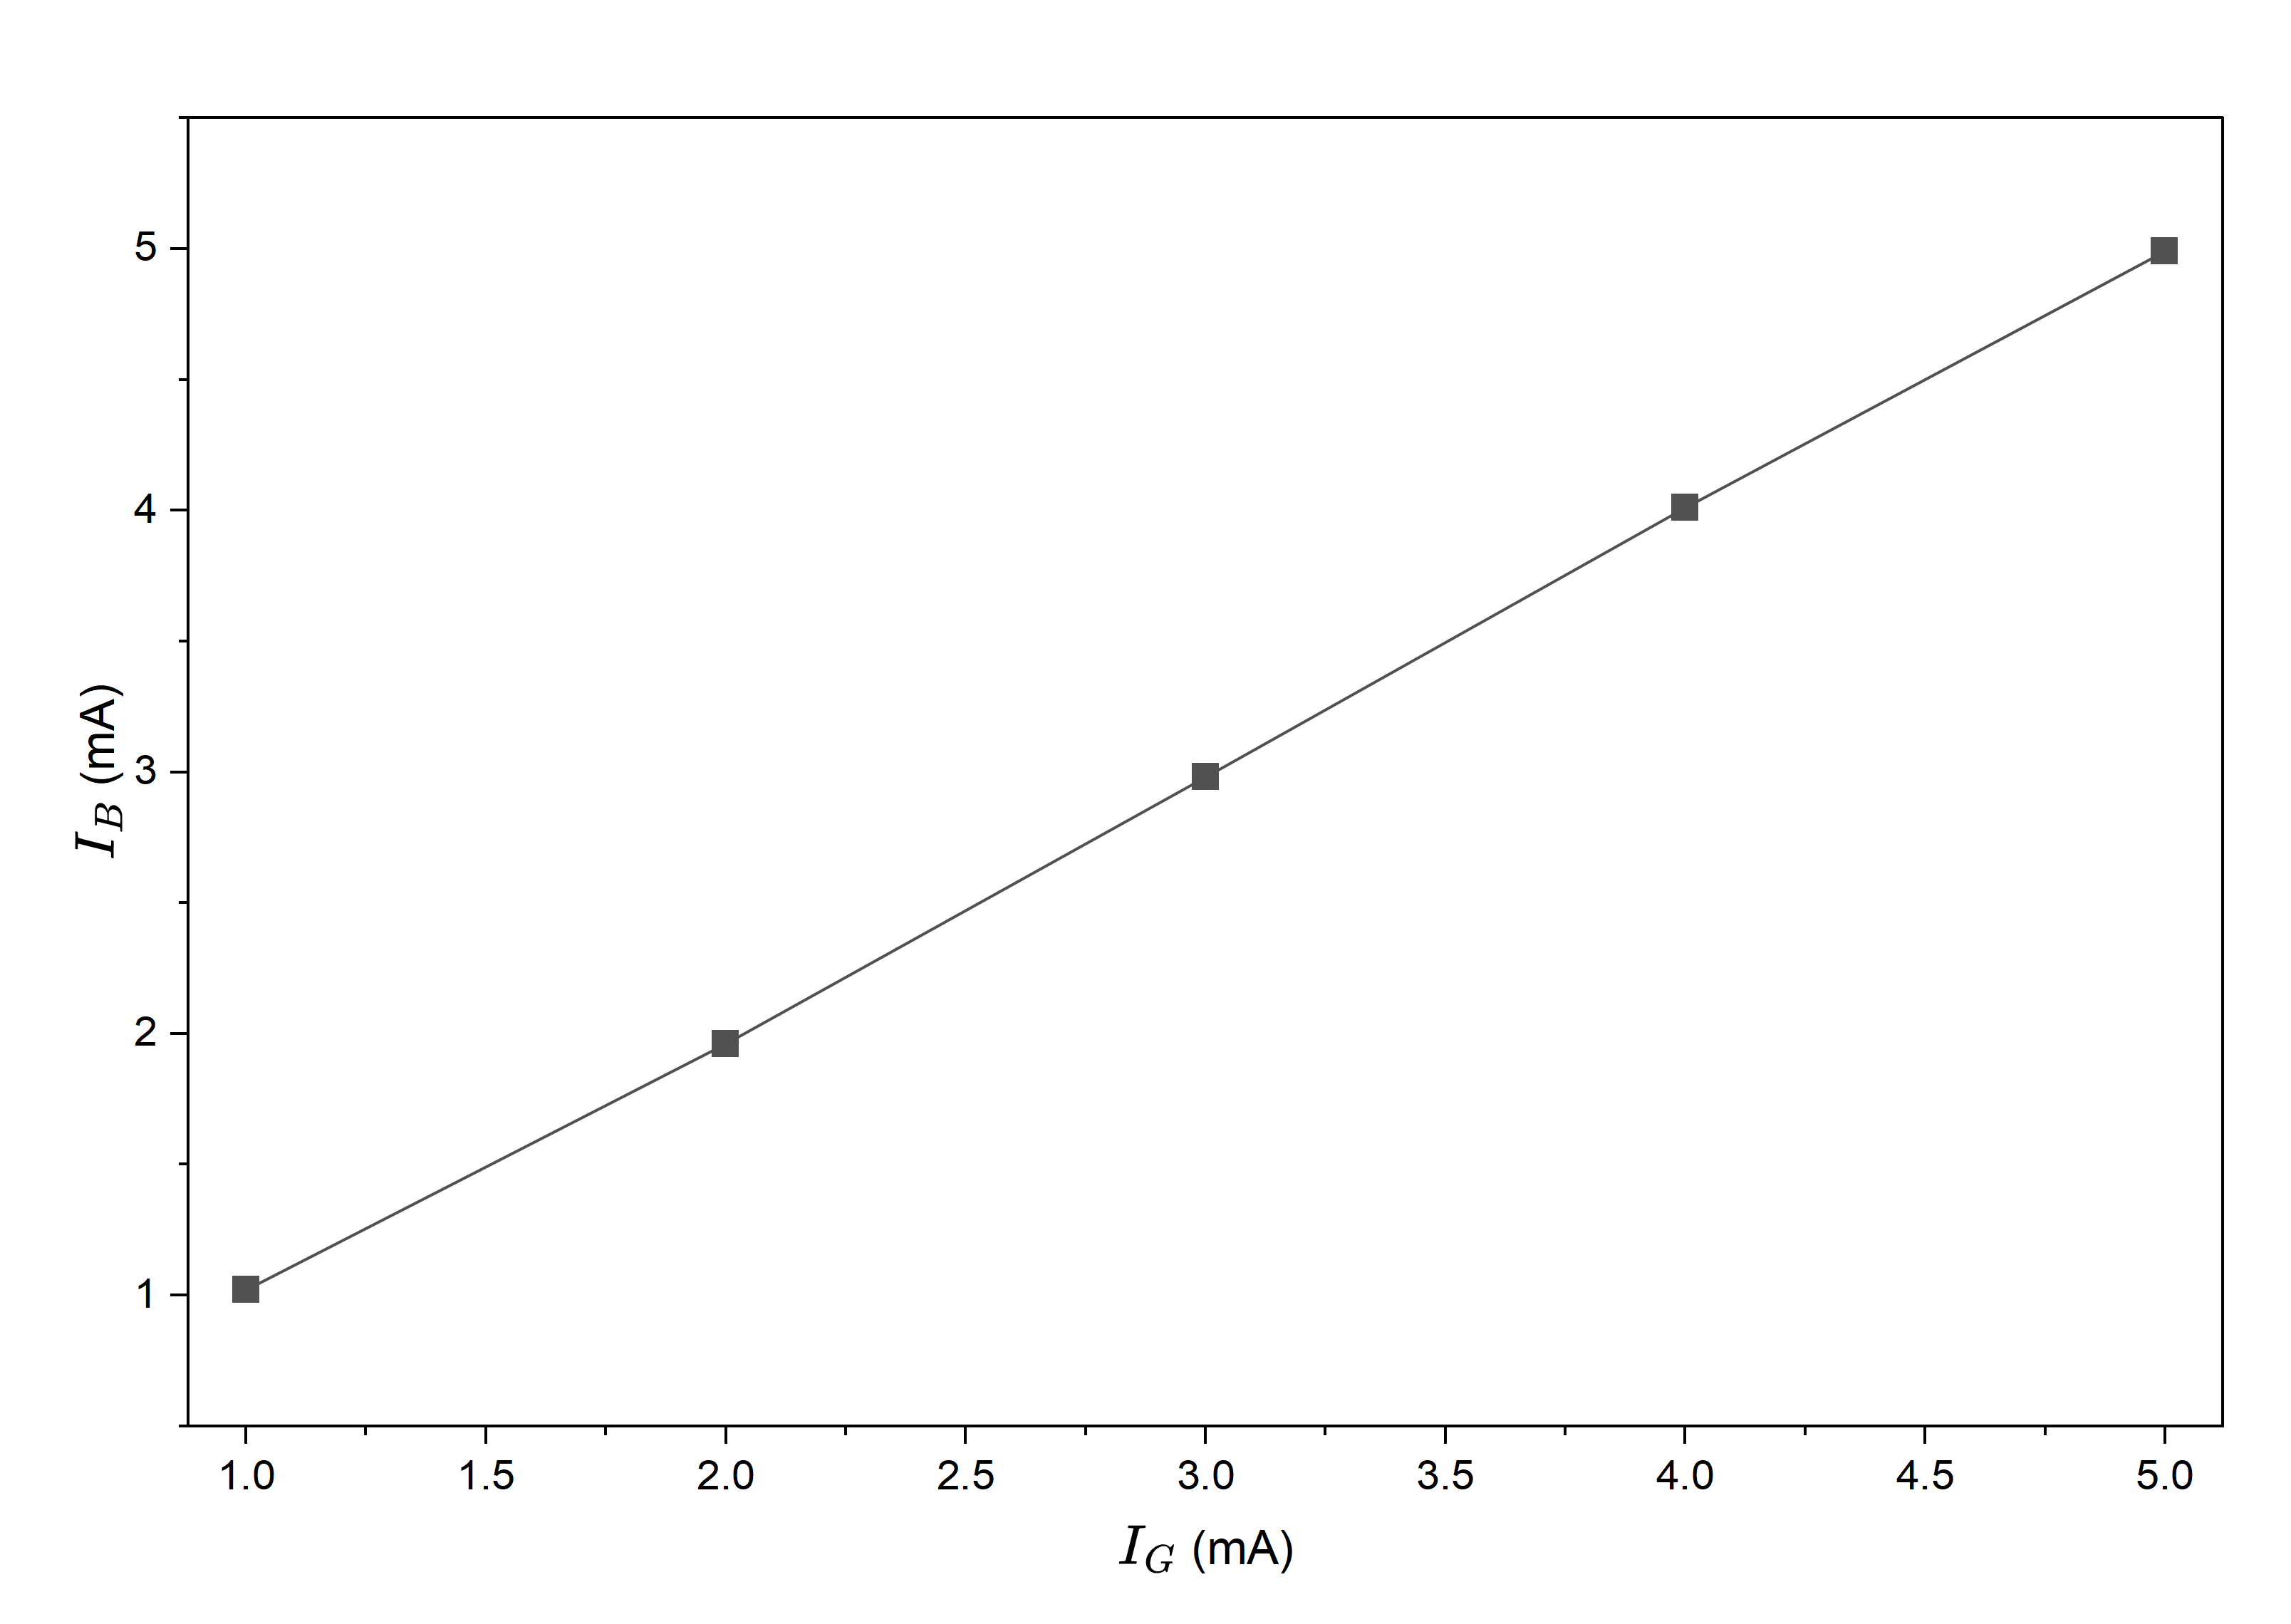
\includegraphics[width=\textwidth]{relaA.png}
        \caption{改装$\SI{5}{\milli A}$电流表的$I_G \sim I_B$曲线}
        \label{graphA}
    \end{subfigure}
    \hfill
    \begin{subfigure}[b]{0.45\textwidth}
        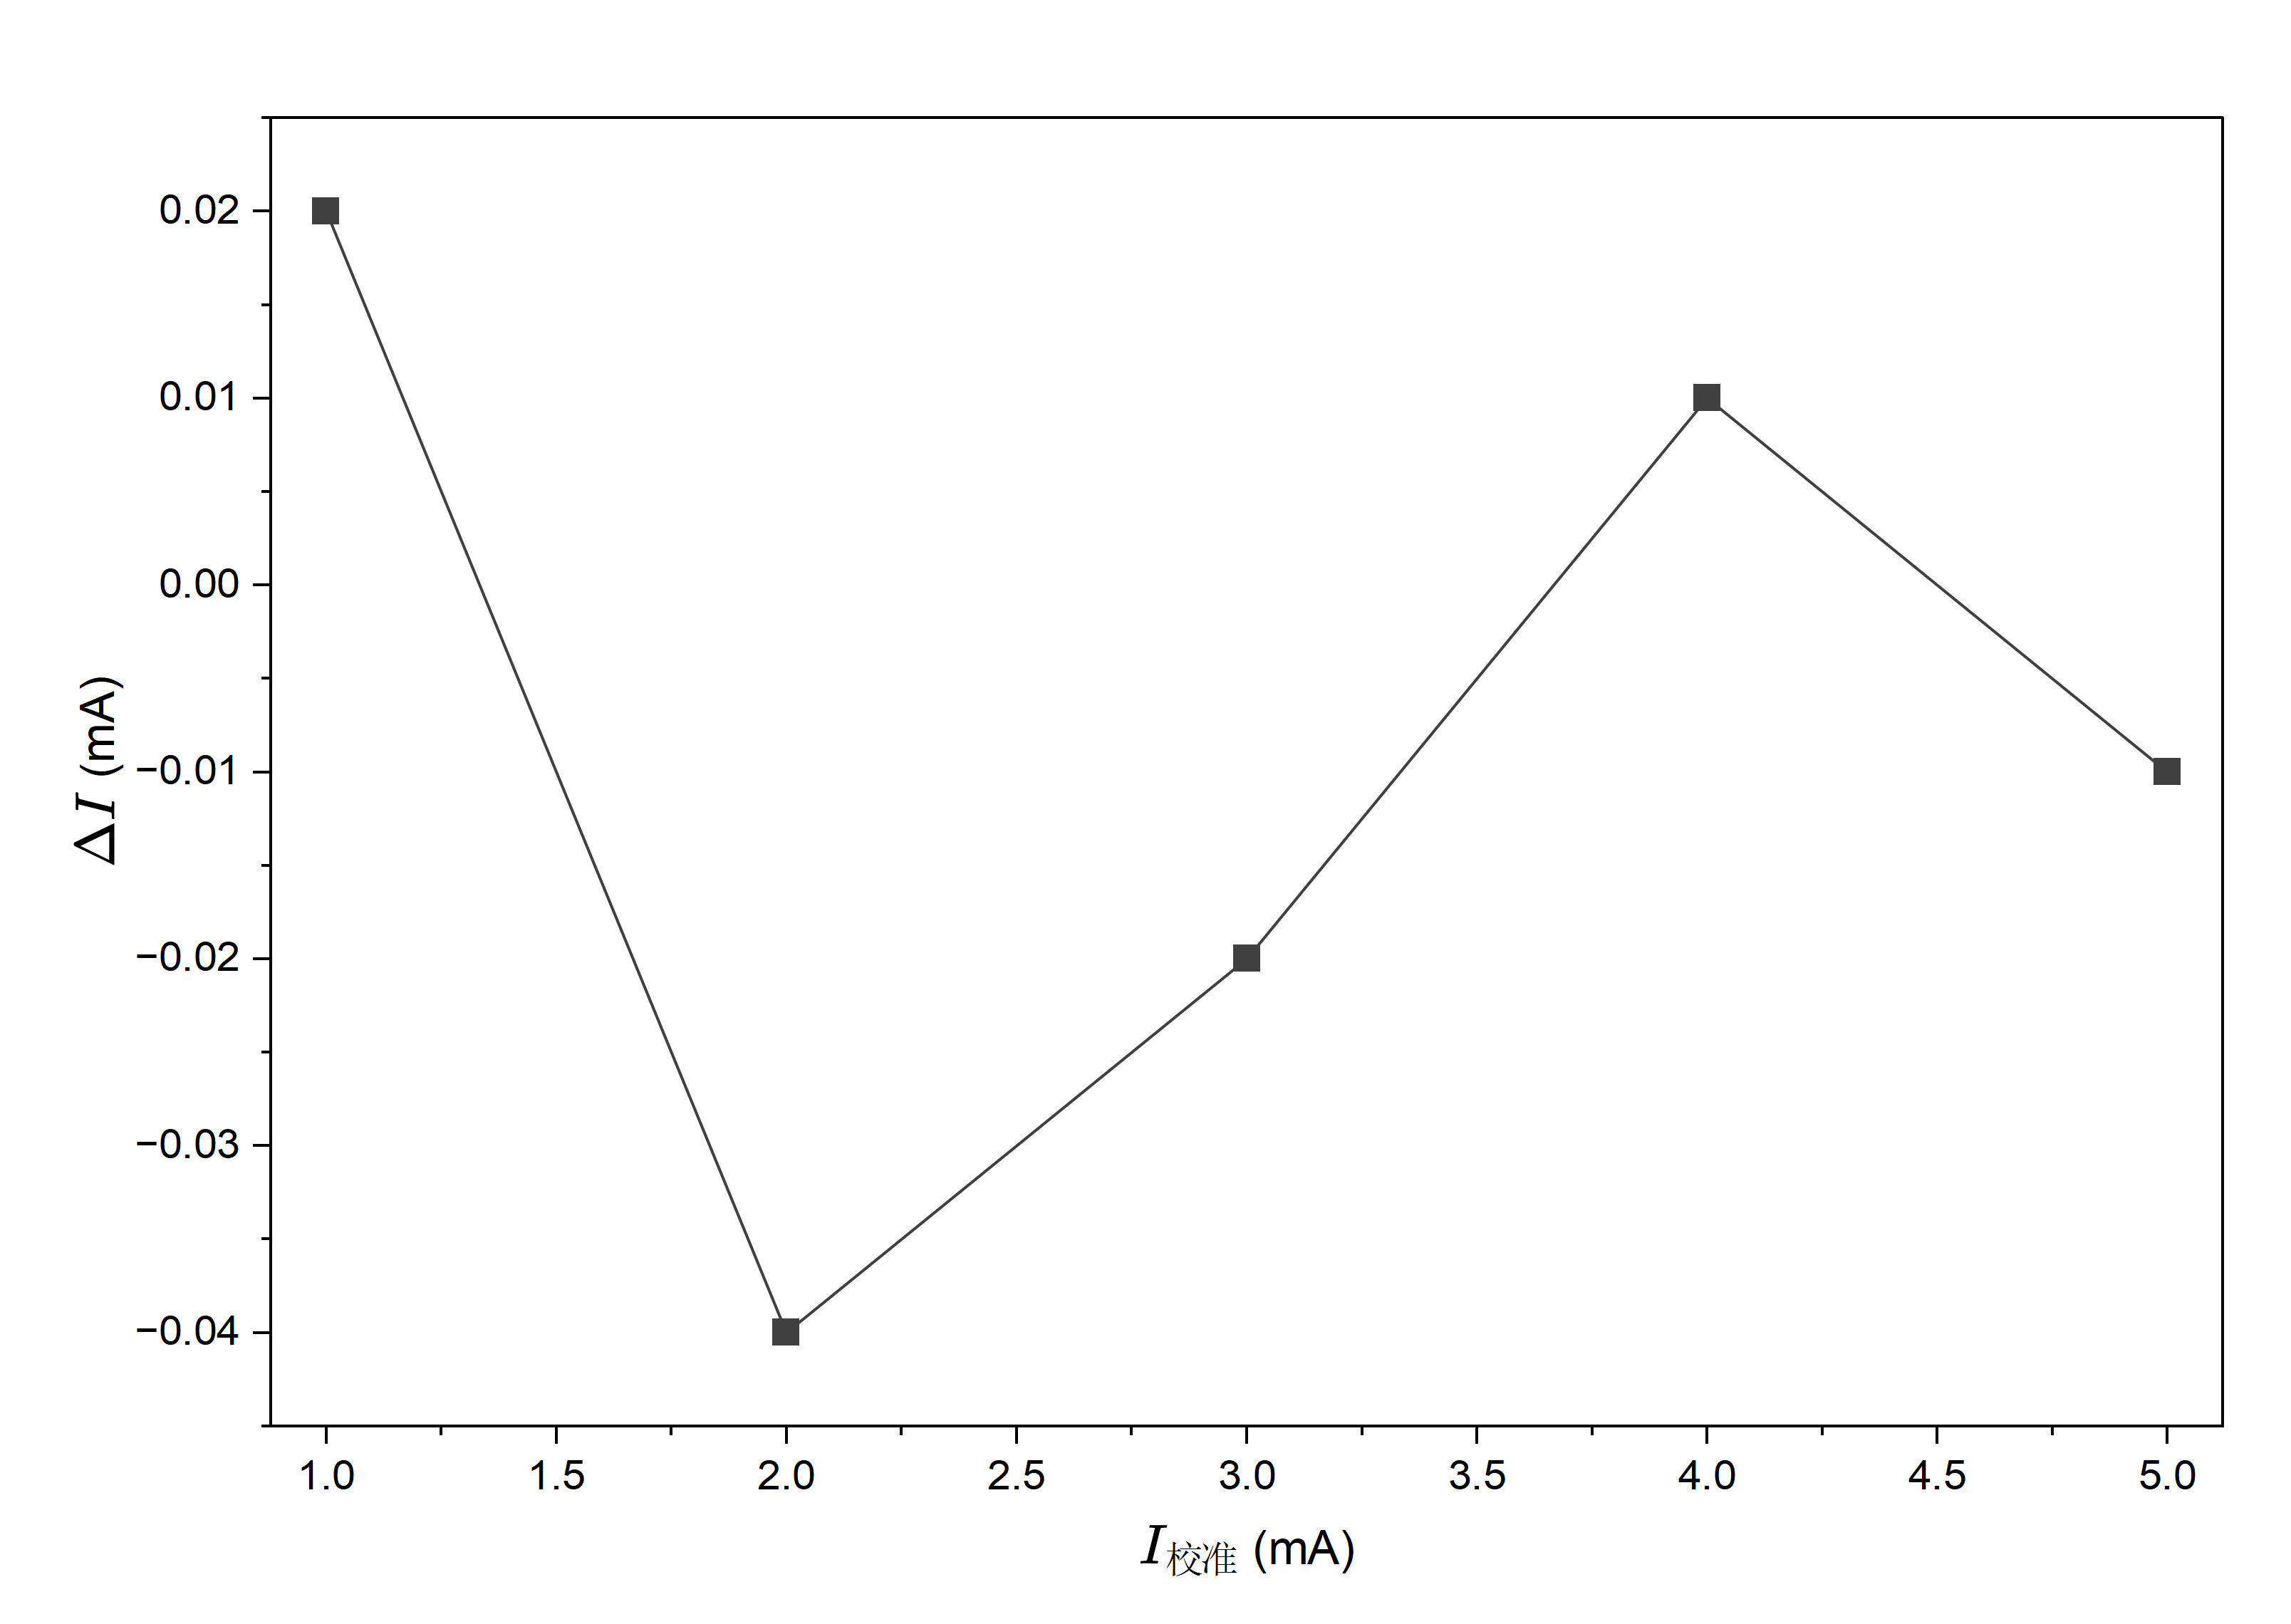
\includegraphics[width=\textwidth]{deltaA.png}
        \caption{改装$\SI{5}{\milli A}$电流表的$\Delta I \sim I_\text{校准}$曲线}
        \label{deltaA}
    \end{subfigure}
    \caption{改装电流表实验数据图}
\end{figure}

\subsubsection{设计、改装并校准电压表}
经计算,$R_3 = \SI{953.8}{\ohm}$。由于改装后电压表分度值为$\frac{\SI{5}{V}}{5 \times 10} = \SI{0.1}{V}$,因此估读到$\SI{0.01}{V}$。实验数据如\cref{tableV}所示,其中$\Delta U = U_{\text{标准}} - U_{\text{改装}}$。
\begin{table}[H]
  \centering
  \caption{改装$\SI{5}{V}$电压表的实验数据}
  \begin{tabular}{C{.3\textwidth} *{5}{C{.11\textwidth}}}
    \toprule
    实验序号 & 1 & 2 & 3 & 4 & 5 \\
    \midrule
    $V_{\text{G}} / \si{V}$ & 1.00 & 2.00 & 3.00 & 4.00 & 5.00 \\
    \midrule
    $V_{\text{B}} / \si{V}$ & 0.95 & 2.01 & 3.02 & 3.99 & 4.99 \\
    \midrule
    $\Delta V / \si{V}$        & -0.05 & 0.01 & 0.02 & -0.01 & -0.01 \\
    \midrule
    $\varepsilon_r$ & 5.00\% & 0.50\% & 0.67\% & 0.25\% & 0.20\% \\
    \midrule
    校准后的串联电阻$R_3 \si{\ohm}$ & 966.7 & 966.7 & 966.7 & 966.7 & 966.7 \\
    \bottomrule
    \label{tableV}
  \end{tabular}
\end{table}
计算得$\Delta_{max} = \left| \frac{0.05}{0.1}\right| = 0.5$,故改装电压表的等级为0.5。
改装后电压表的$V_G \sim V_B$曲线如\cref{relaV}所示,$\Delta V \sim V_\text{校准}$曲线如\cref{deltaV}所示。
\begin{figure}[htbp]
    \centering
    \begin{subfigure}[b]{0.45\textwidth}
        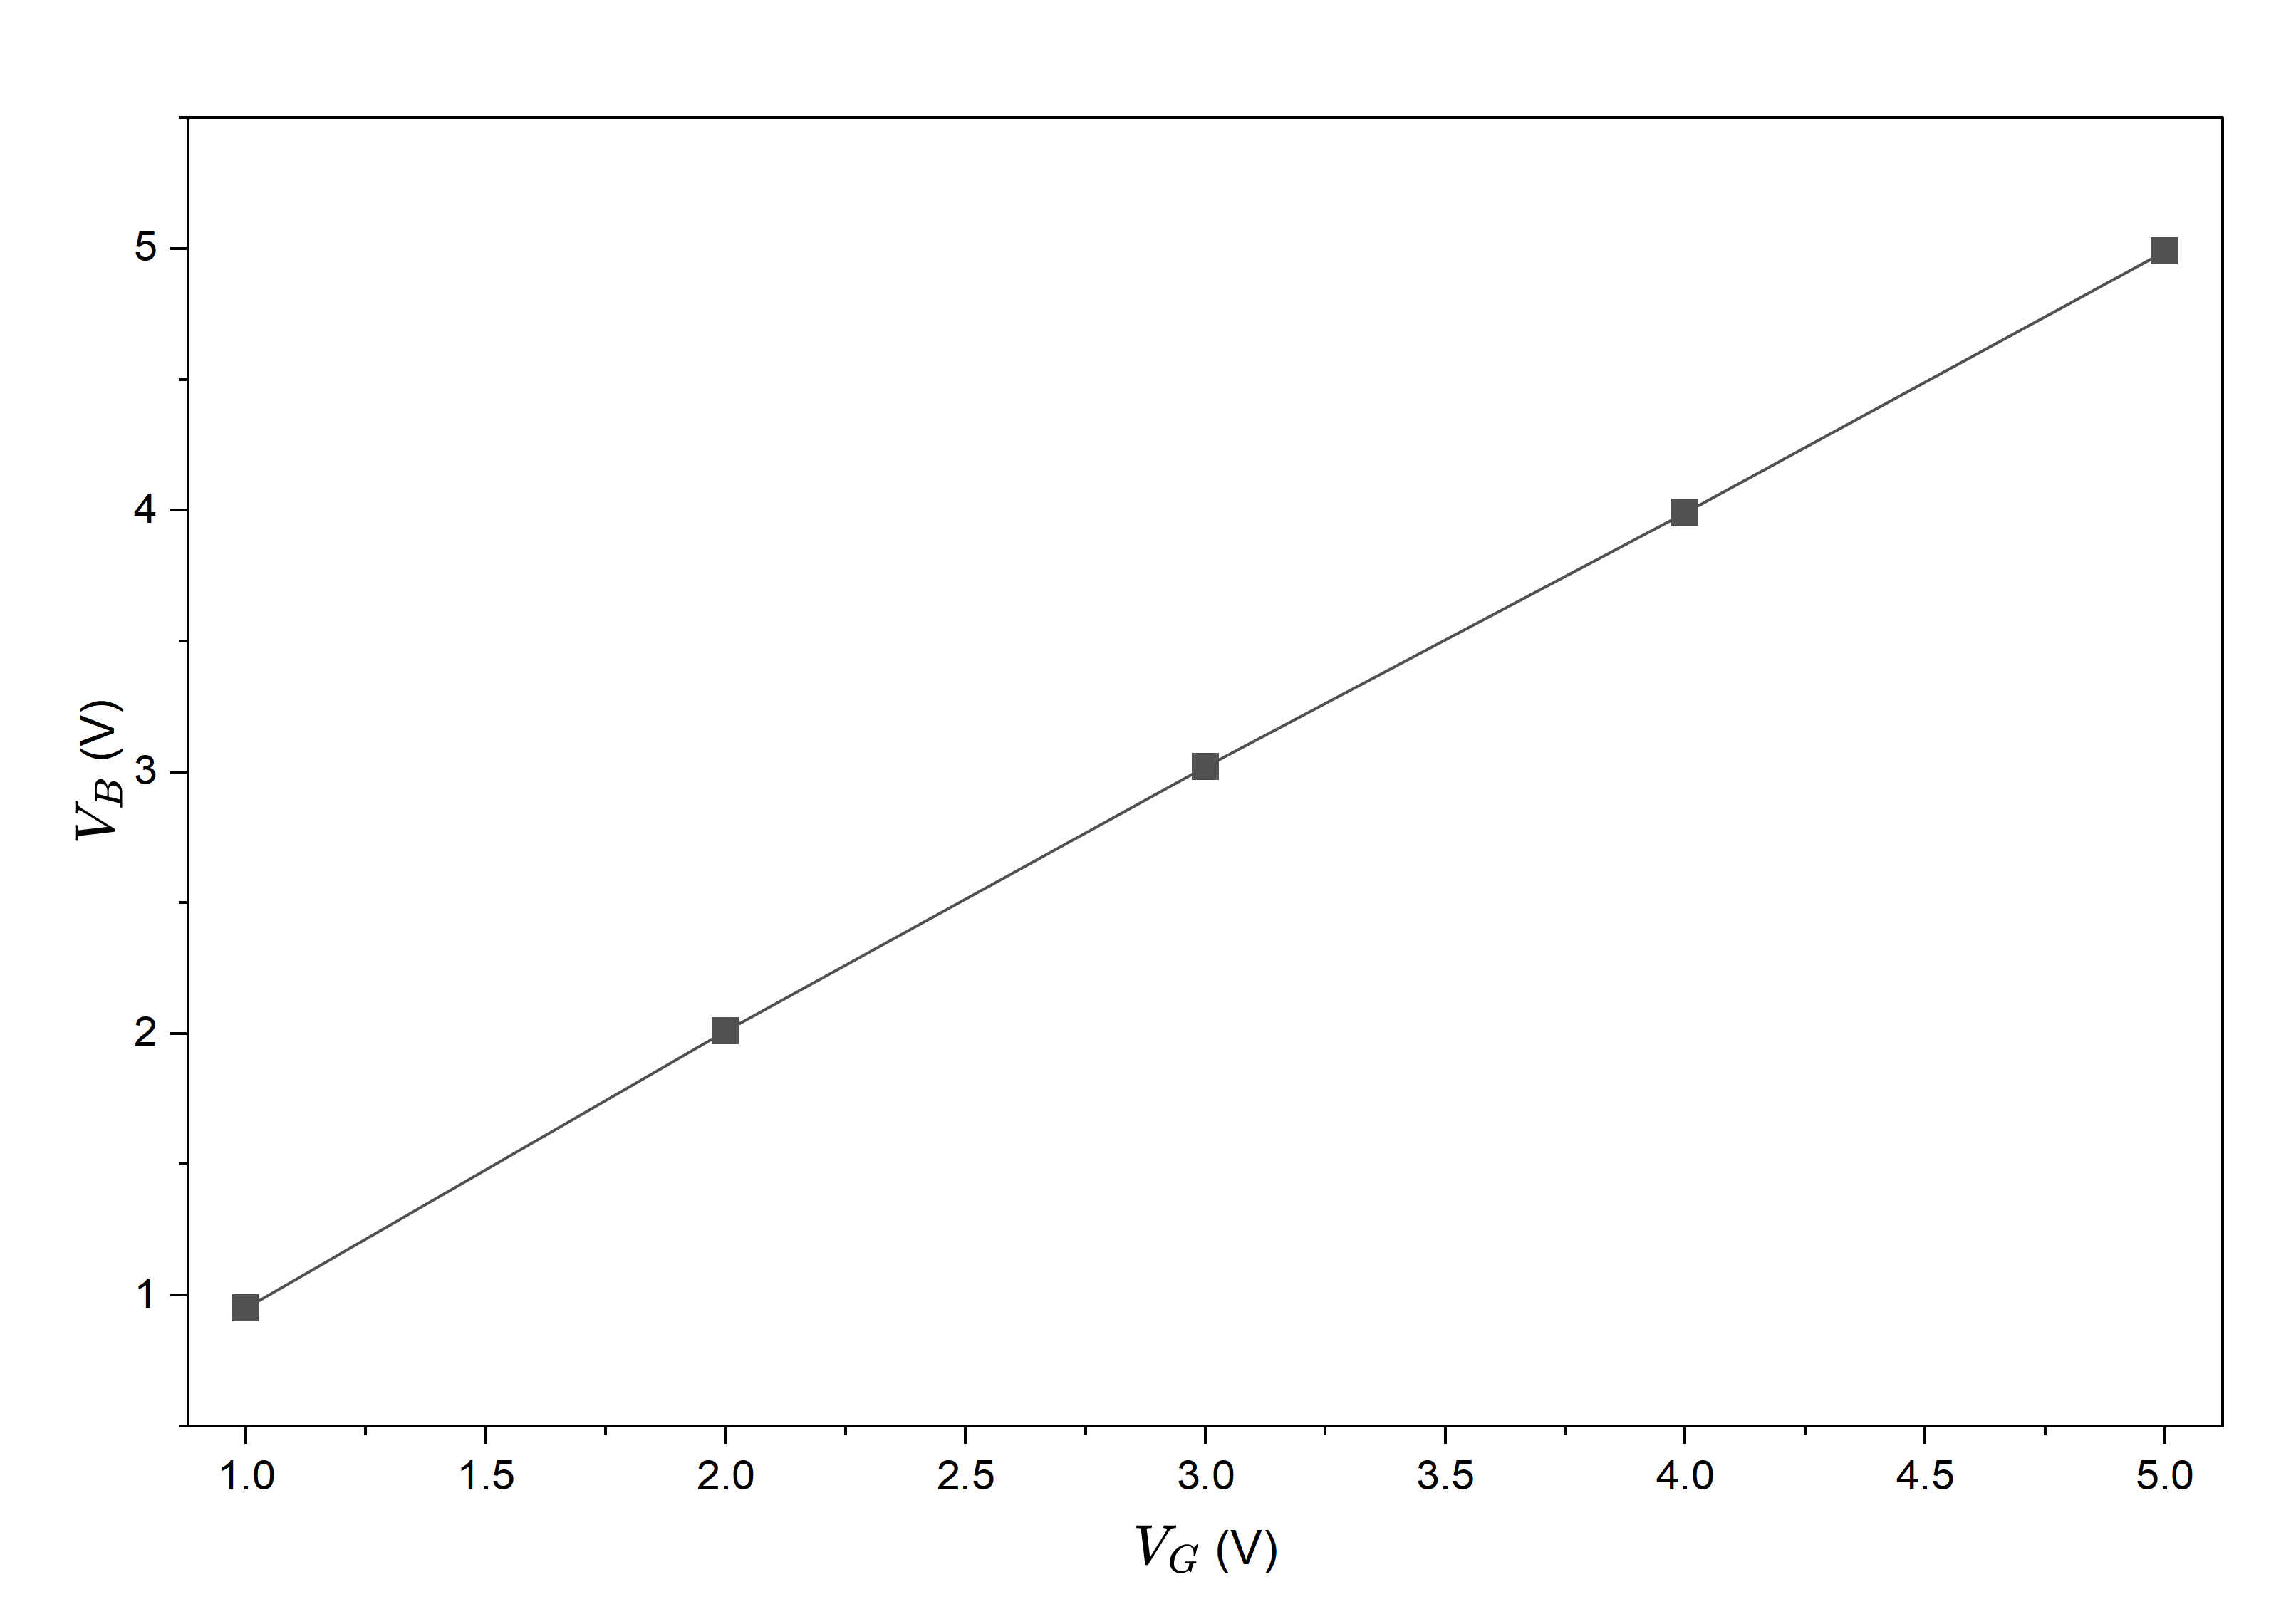
\includegraphics[width=\textwidth]{relaV.png}
        \caption{改装$\SI{5}{V}$电流表的$V_G \sim V_B$曲线}
        \label{relaV}
    \end{subfigure}
    \hfill
    \begin{subfigure}[b]{0.45\textwidth}
        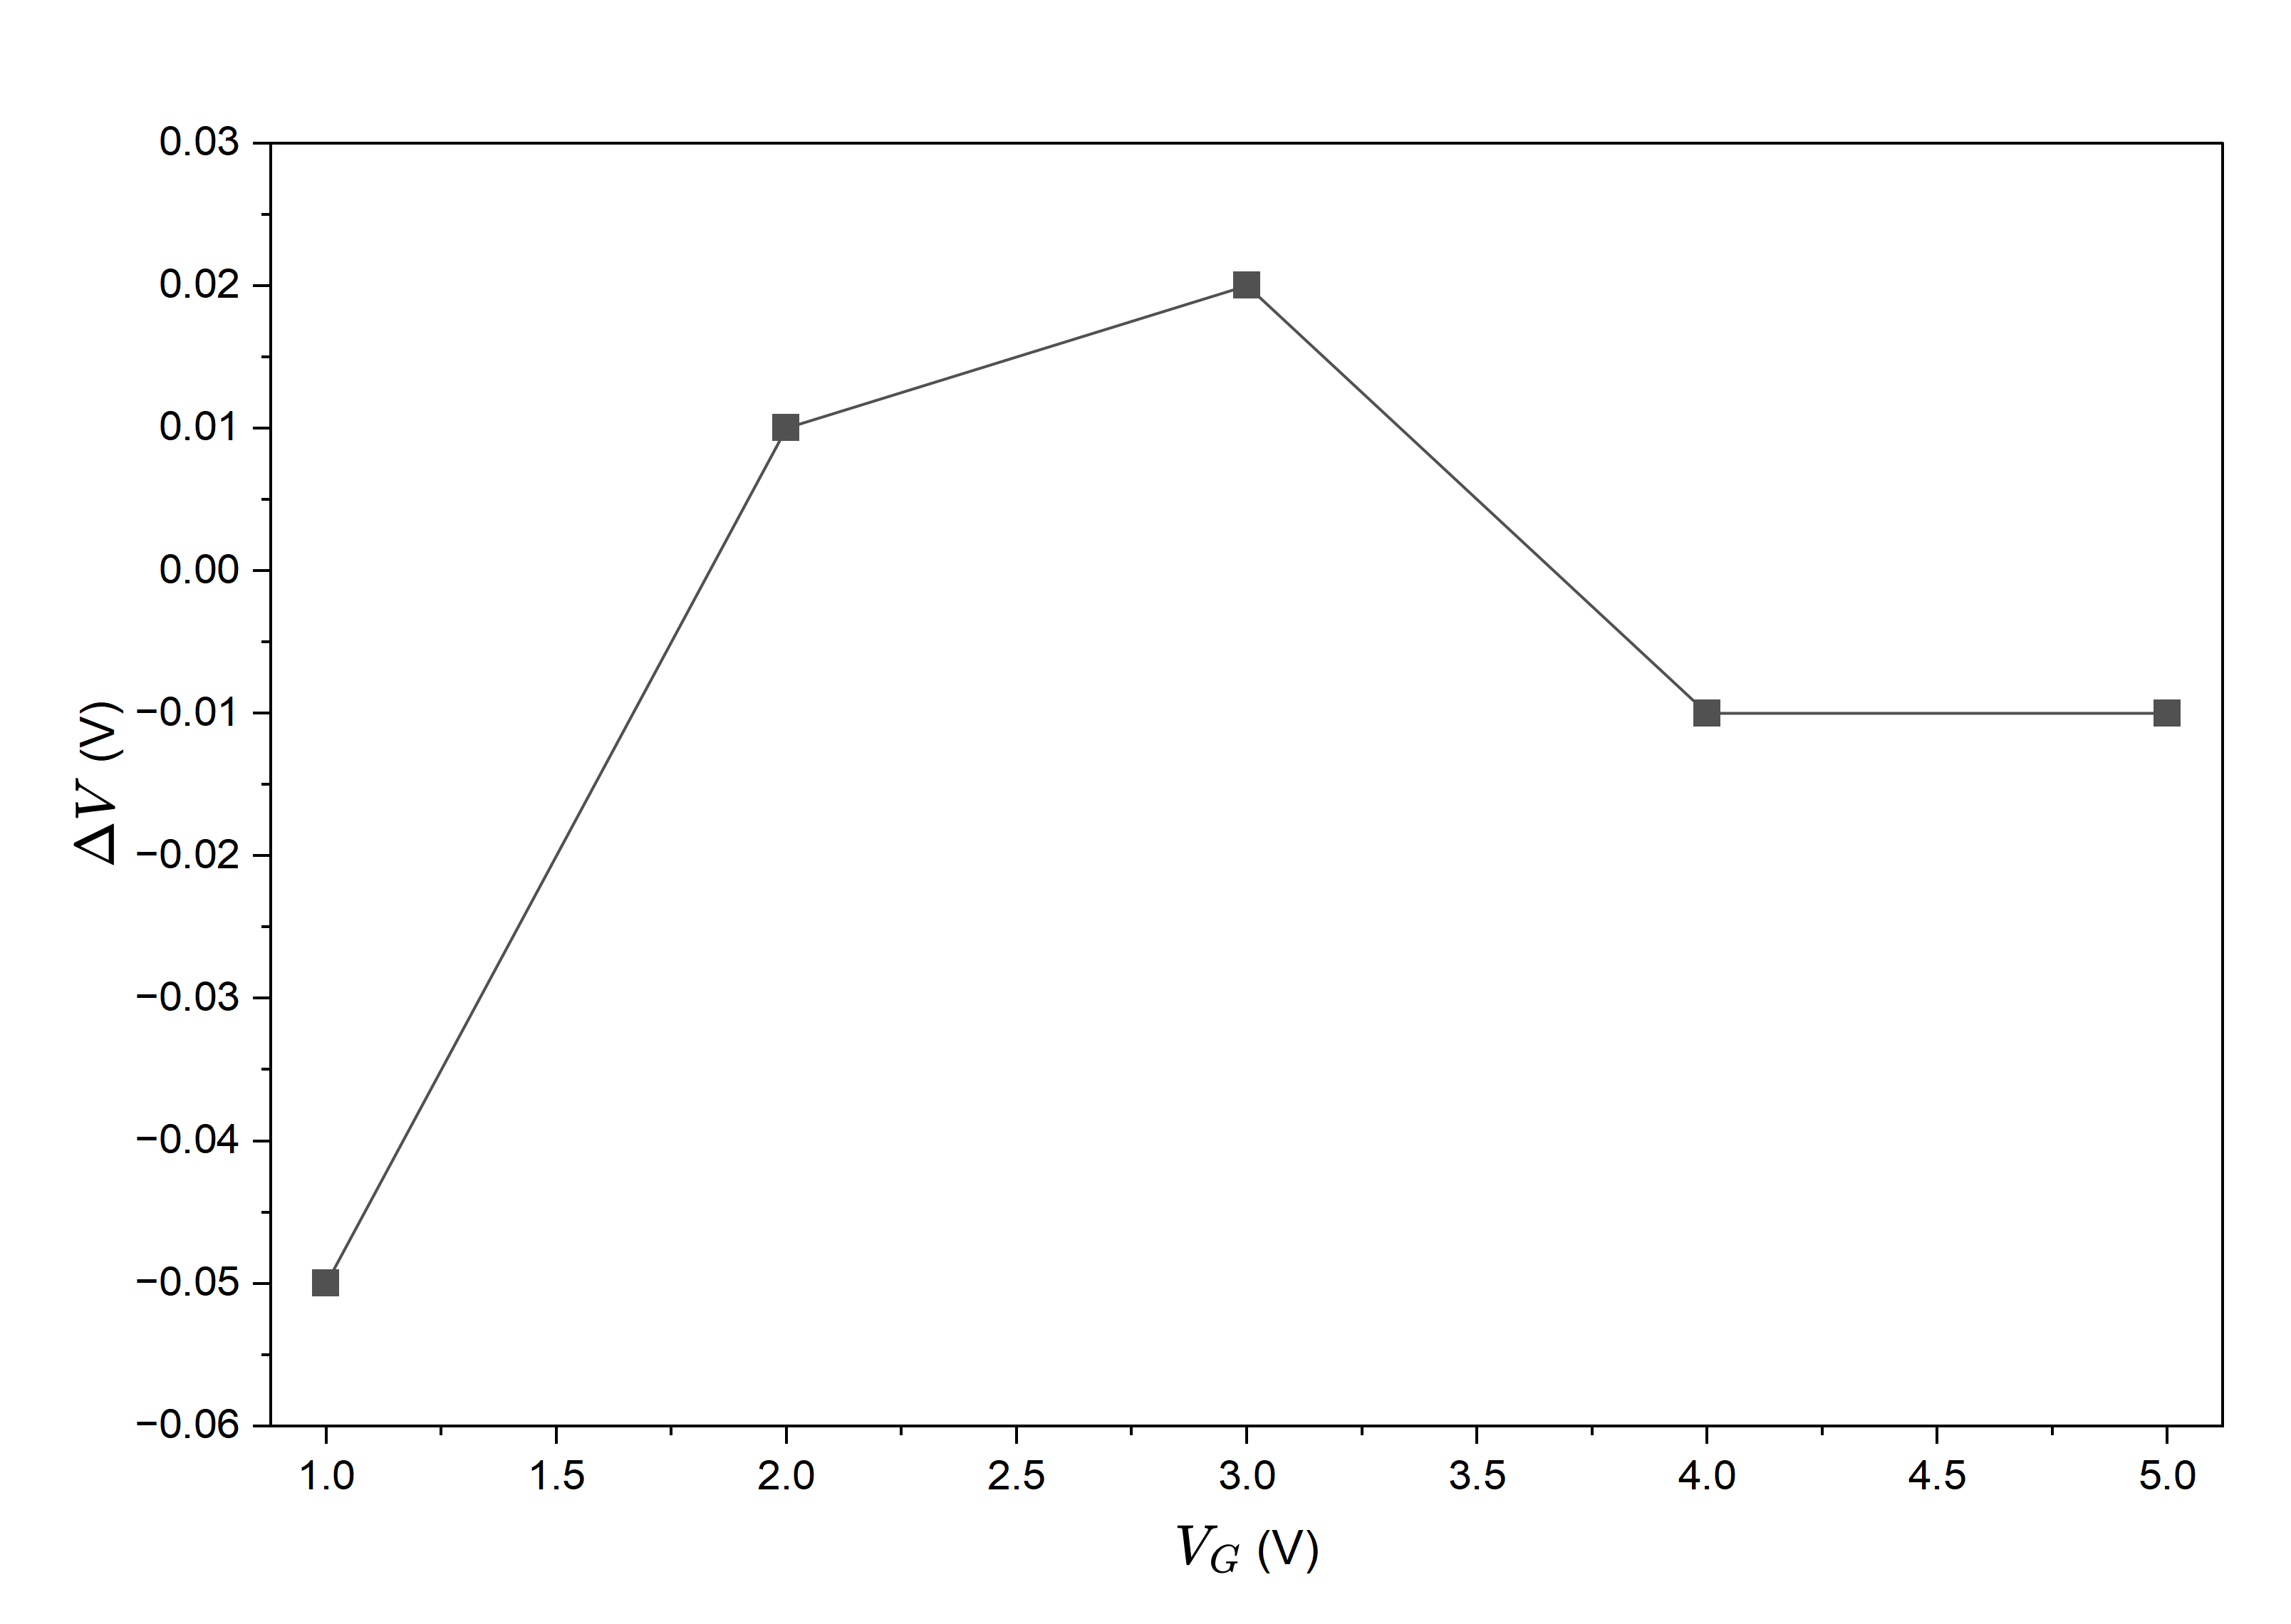
\includegraphics[width=\textwidth]{deltaV.png}
        \caption{改装$\SI{5}{V}$电流表的$\Delta V \sim V_\text{校准}$曲线}
        \label{deltaV}
    \end{subfigure}
    \caption{改装电压表实验数据图}
\end{figure}

\subsubsection{设计并改装欧姆表}
首先,欧姆调零,调零后$R_6 = 30.5 \si{\ohm}$。再调整电阻箱至欧姆表电流为满偏的一半,读出中值电阻为$R_\text{中值} = 284.6 \si{\ohm}$。
记录实验数据如\cref{tableOhm}。
\begin{table}[H]
  \centering
  \caption{改装欧姆表的实验数据}
  \begin{tabular}{C{.1\textwidth} *{13}{C{.04\textwidth}}}
    \toprule
    实验序号 & 1 & 2 & 3 & 4 & 5 & 6 & 7 & 8 & 9 & 10 & 11 & 12 & 13\\
    \midrule
    $I_x(\si{mA})$ & 0.744 & 0.662 & 0.594 & 0.537 & 0.481 & 0.443 & 0.418 & 0.391 & 0.360 & 0.321 & 0.284 & 0.260 & 0.239 \\
    \midrule
    $R_x(\si{\ohm})$ & 100.0 & 150.0 & 200.0 & 250.0 & 300.0 & 350.0 & 400.0 & 450.0 & 500.0 & 600.0 & 700.0 & 800.0 & 900.0 \\
    \bottomrule
    \label{tableOhm}
  \end{tabular}
\end{table}
作出$I_x \sim R_x$曲线如\cref{graphOhm}所示。
\begin{figure}[htbp]
        \centering
        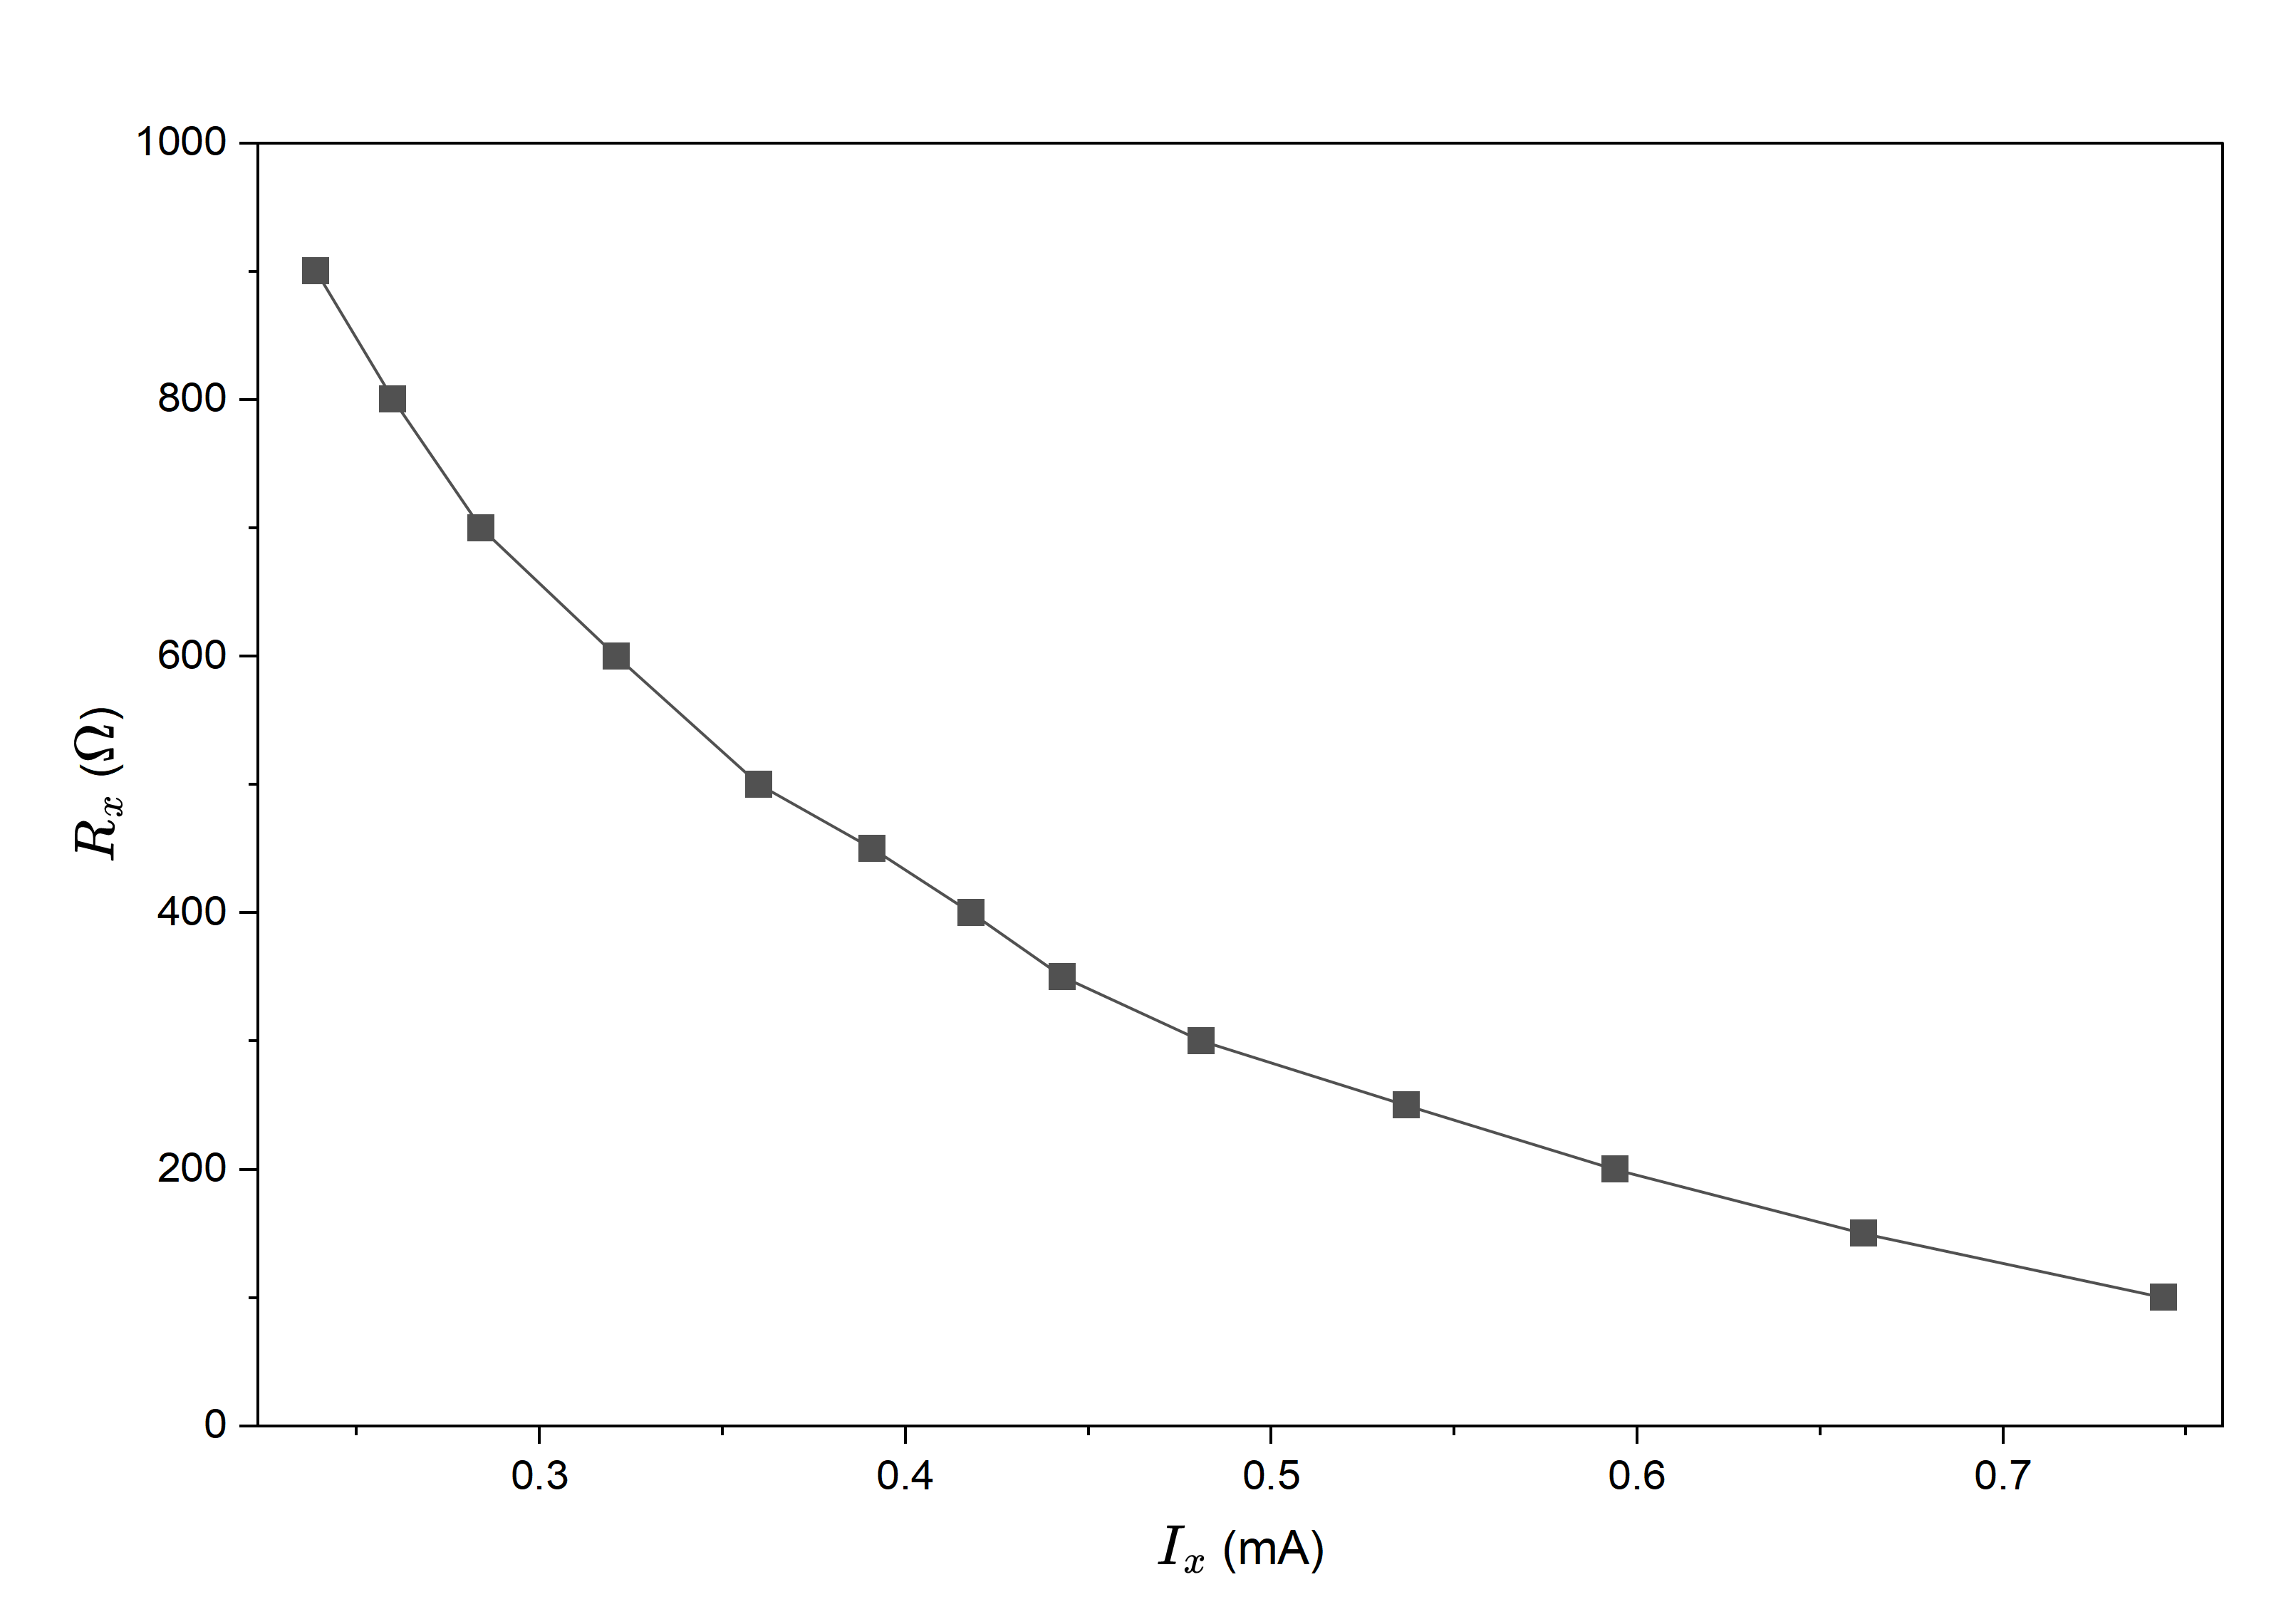
\includegraphics[width=0.4\textwidth]{graphOhm.png}
        \caption{改装欧姆表的$I_x \sim R_x$曲线}
        \label{graphOhm}
\end{figure}
可见,欧姆表的示数随通过的电流增大非线性地减小,而且,通过的电流越大,减小的速率就越缓。即,在欧姆表表盘上,最大电流刻度为$\SI{0}{\ohm}$,最小电流刻度为$\infty\si{\ohm}$,从右往左电阻示数依次增大;电阻间隔一致时,刻度间隔左密右疏。

\subsection{误差分析}
三个实验的绝对误差、相对误差已经在对应表格列出。本次实验每个数据都只测量了一次,因此不计算标准误差和A类不确定度。根据以上讨论,可以知道改装电流表的B类不确定度为${u_b}_A = \frac{\Delta_\text{仪}}{\sqrt{3}} = \frac{0.04}{\sqrt{3}} \si{mA} = 0.023 \si{mA}$,改装电压表的B类不确定度为${u_b}_V = \frac{\Delta_\text{仪}}{\sqrt{3}} = \frac{0.05}{\sqrt{3}} \si{V} = 0.029 \si{V}$。

以下是本实验误差的主要来源:
\begin{enumerate}
    \item 实验所用电流计、标准电流表、标准电压表精度有限,结果精度低。特别是电表校准时,调节相应电阻的十位和个位数,电表示数几乎没有变化;
    \item 由于表盘较小、表针较粗,读数时视线不可能严格垂直表盘,读数存在视差;
    \item 实验中标准电表和表头指针存在持续的跳动现象,影响读数;
    \item 实验仪器的各项参数可能与标称值存在一定差别;
    \item 每个实验数据只测量了一次,存在一定偶然误差。
\end{enumerate}

\subsection{实验探讨}
本次实验回顾了高中物理中制作万用表的知识,并以此为基础使我掌握了大学物理实验的规范和数据处理方法。尽管原理并不复杂,实际操作中也会遇到各种预想不到的问题,让我深刻意识到物理是一门实验科学,理论与实践相辅相成。

\section{思考题}
\begin{enumerate}
    \item 为什么不能用万用表欧姆档测量电源内阻?

        首先,从原理上说,欧姆表是由$\frac{\varepsilon}{I_g}$的若干倍来标称电阻的,当外接电源时,分子就不再是欧姆表内置电源的电动势$\varepsilon$,而是$\varepsilon$与外接电源的电动势之和(差),因此结果是错误的。
        其次,欧姆表的满偏电流和内置电源电压都比较小,若外接电源电压较大,或者反接,可能会使欧姆表超量程乃至损坏。

    \item 为什么不能用欧姆表测量另一表头内阻?

        首先,表头电阻较小,而欧姆表测量精度较低,测量误差比较大;
        其次,表头允许流过的电流很小,而欧姆表测量时,电流较大,可能会损坏表头。
        如果确需测量,可以串联一个电阻箱,调整其阻值使该支路总阻值约为中值电阻,用欧姆表测出总阻值,再减去电阻箱阻值,即为表头内阻。

    \item 为什么$I_x$与$R_x$为非线性关系?
    
        根据\cref{gaizhuangOhm}电路结构和闭合电路欧姆定律,我们知道$I_x = \frac{\varepsilon}{R_g' + R' + R_x}$,其中$\varepsilon, R_g', R'$均为常数,因此$I_x$与$R_x$的关系为反比例函数,显然是非线性的。   
\end{enumerate}
\end{fullreportonly}
\insertnotes
\end{document}
